\documentclass[12pt]{article}
\usepackage[utf8]{inputenc}
\pagenumbering{arabic}
\usepackage{graphicx}
\usepackage{amstext}
\graphicspath{ {images/} }


\begin{document}

\begin{titlepage}
    \begin{center}
    \begin{figure}
        \centering
        
\includegraphics[scale=0.2]{logoPolimi.png}
        \vspace{1.5cm}
    \end{figure}

    \Huge\textbf{Software Engineering 2 Project - Travlendar+}
    \rule{12cm}{0.5pt}
    \Huge\textbf{RASD - Requirement Analysis and Specification Document}
    \today
    \end{center}
    
    \vspace{3cm}
    
    \begin{flushleft}
        \LARGE\textbf{Authors: }
        \newline\newline
        \Large\texttt{}{Francisco Cristóvão \\ Samsom Beyene}
    \end{flushleft}



\end{titlepage}

\newpage
  \tableofcontents
\newpage

\section{Introduction}
\subsection{Purpose}
The main goal of this project is to create a calendar-based application that provides the user a convenient way of organizing his/her daily schedule, maximizing its productiveness and minimizing the worthless time of his/her day. With this in mind, the application:
\begin{itemize}
\item computes and accounts for travel time between appointments
\item supports the user in his/her travels
\end{itemize}

\subsection{Scope}
The Travlendar+ is  a calendar based application which helps people to schedule appointments in flexible and fully -featured calendar support by considering the travel time between meetings. The application supports a multitude of travel means, including walking, biking, public transportation, and driving. The application is dynamic in order to support weather forecast. A particular user may globally activate or deactivate each travel means ((e.g., a user who does not own a bicycle would deactivate biking). A user can also be able to provide reasonable constraints on different travel means (e.g., walking distances should be less than a given distance, or public transportation should not be used after a given time of day). 
Specifically  when a user interacts with the application ,the application can: compute travel times between meetings (or proposed meetings) and prevent scheduling meetings whose start/end times conflict as a result of inability to travel, explicitly but subtly add "travel time" to the calendar between meetings, reserving the required amount of time on the calendar, suggest  the "best" option of travel between each meeting, create overall compatible schedules on a day-basis by considering that a user who does not leave the house with his bicycle or car in the morning cannot use it to move between meetings during the day, and specify a flexible “lunch” with a minimum of 30 minutes within the specified time of the day(11:30-2:30).
The Travlendar+ application supports different types of users, including people who work "on the road", traveling from meeting to meeting throughout the day as well as busy parents shuttling kids to and from.( In this part we have to add what the system (application) needs to function).

\subsection{Definitions, Acronyms, Abbreviations}

\subsection{Revision History}

\subsection{Reference Documents}
Assignment document: Mandatory Project Assignments.pdf

\subsection{Document Structure}
Other than this introductory chapter, this RASD is organized in five more chapters. Chapter two is meant to provide an overview of the systems functionalities, the type of users it is meant for and the different kinds of interactions it contemplates, not only with the users themselves, but also with other systems. Some of the systems requirements are also slightly discussed in this chapter, even though they’ll be analysed in the following chapter. In the third chapter (as mentioned above) the systems requirements, attributes and constraints are analysed and discussed with the appropriate detail and depth, specifying exactly how they should be.
The fourth chapter deals with the formal analysis of the system using and Alloy model. It includes the Alloy model of the system, with a brief discussion on its purpose and on the relevance of using Alloy as a tool to validate our solution, given the problem we had to solve.
In the fifth chapter the effort spent by each of the group members is described by specifying the number of hours each member of the group worked on the development of this document.

\section{Overall Description}

\subsection{Product Perspective}
    \begin{figure}[ht]
        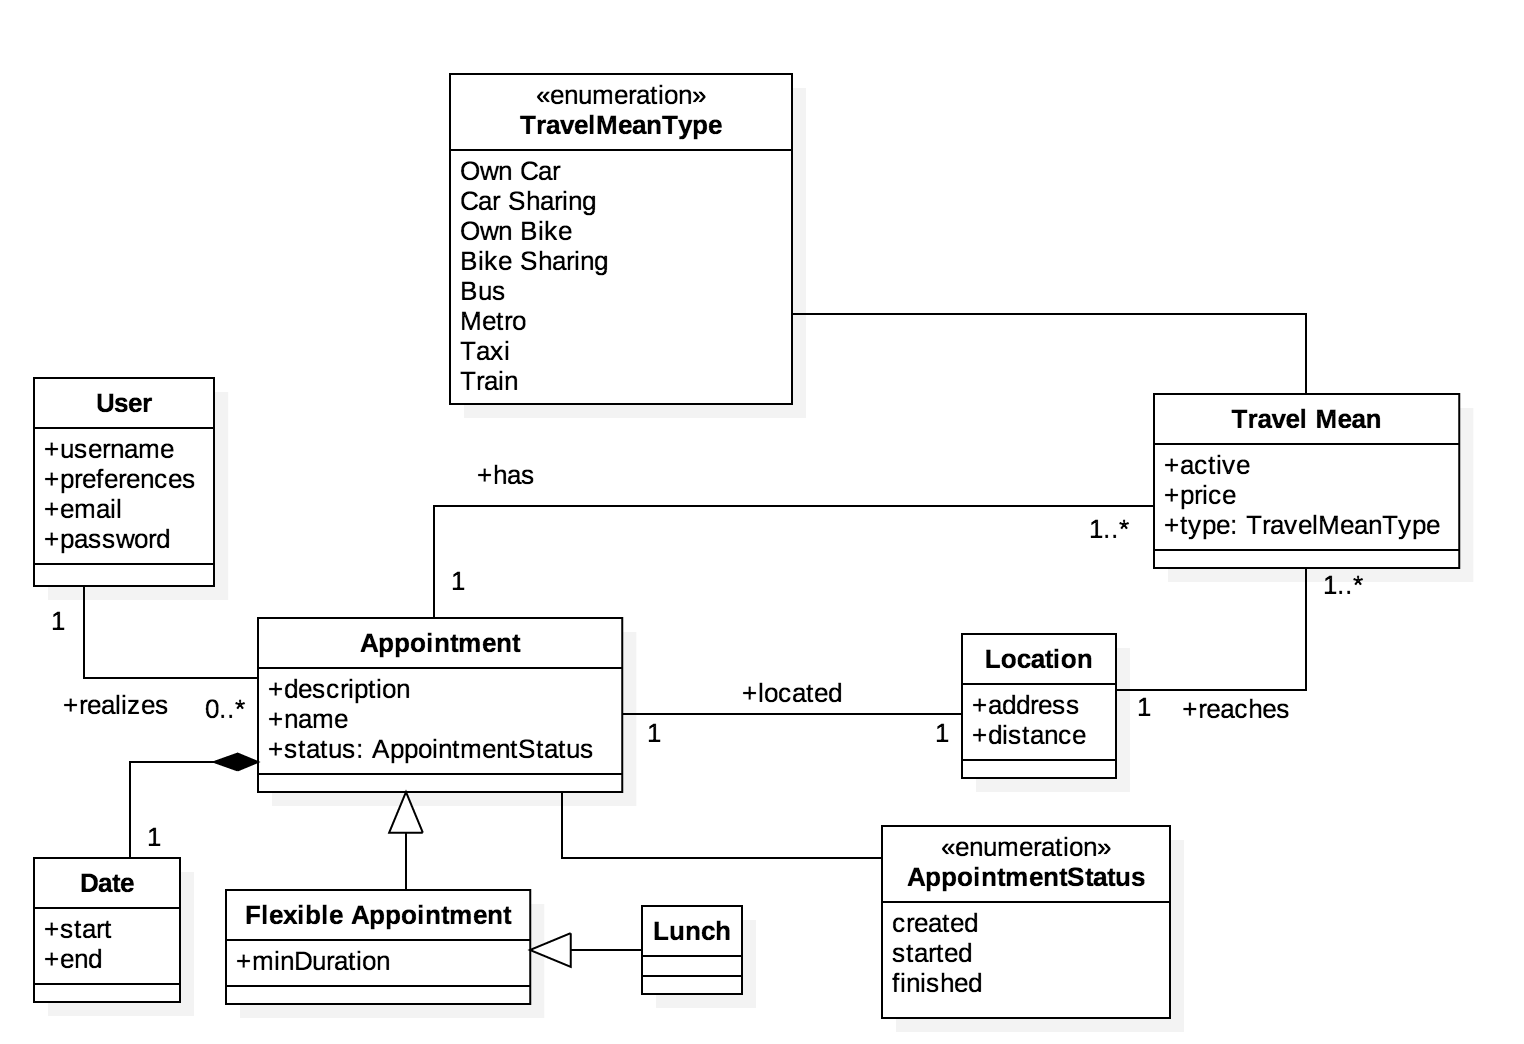
\includegraphics[scale=0.52]{domainModel.png}
        \caption{Class Diagram of the domain}
    \label{fig:domainModel}
    \end{figure}

\end{document}
